\documentclass{article}
\usepackage{longtable}
\usepackage{makecell}
\usepackage{float}
\usepackage{graphicx}
\usepackage{bm}
\usepackage{placeins}
\usepackage{booktabs}
\usepackage{gensymb}
\usepackage{amssymb}
\usepackage{indentfirst}
\usepackage{threeparttable} 
\usepackage{multirow}
\usepackage{aligned-overset}
\usepackage[slantfont,boldfont]{xeCJK}
\usepackage{fontspec}
\renewcommand{\arraystretch}{1.5}
\usepackage[paperwidth=20cm,paperheight=33.3cm]{geometry}
\setCJKmainfont{SimSun}
\setmainfont{SimSun}
\setsansfont{SimSun}

\title{数字示波器实验报告}
\author{2411545 邱凯锐}
\date{2025.5.19}

\begin{document}
\maketitle
\section{实验目的}
1.掌握数字示波器(简称DSO)的基本原理和使用方法

2.学会用DSO观察稳压二极管的伏安特性曲线,并测其动态电阻。

3.学会用DSO测量电解电容器的电容。

\section{实验原理}
\subsection{稳压二极管动态电阻的测量}
稳压二极管的伏安特性曲线如Figure 1所示。曲线上任一点P处的电压与电流的比值称为该状态下的静态电阻;该点处的微小电压改变量与相应的电流改变量之比称为该状态下的动态电阻。

\begin{figure}[!ht]
    \centering
    \begin{minipage}{0.45\textwidth} % 调整宽度为总宽度的45%
        \centering
        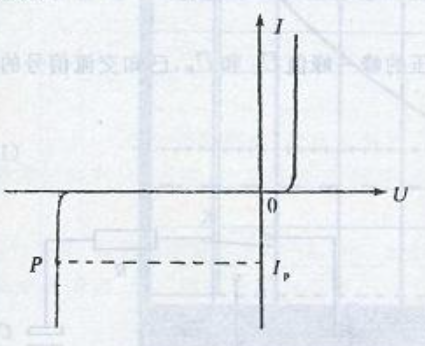
\includegraphics[width=5cm]{1.png} % 替换为你的图片路径
        \caption{稳压二极管伏安特性曲线图}
    \end{minipage}\hfill
    \begin{minipage}{0.45\textwidth}
        \centering
        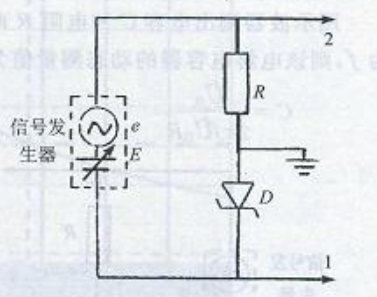
\includegraphics[width=5cm]{2.png} % 替换为你的图片路径
        \caption{稳压二极管动态电阻测量实验电路图}
    \end{minipage}
\end{figure}

按Figure 2连接电路,其中信号发生器的频率为$f$(本实验为$100\ Hz$)。将稳压二极管$D$及电阻$R$两端电压分别输至DSO的1和2通道(即X、Y通道)。操作DSO,可在荧光屏上调出稳压二极管的伏安特性曲线。其形状与Figure 1成左右反转对称,即电压轴正方向指向左方。

调节信号源并结合示波器,将稳压二极管的工作电流$I_P$设置为$-10\ mA$。保持信号源直流调节旋钮不变,缓慢调节信号源交流电压幅度,使得示波器上稳压二极管两端电压的正弦波形恰好不发生畸变,测出稳压二极管$D$和电阻$R$两端正弦波电压的峰-峰值$\widetilde{U_D}$和$\widetilde{U_R}$,即可求出稳压二极管的动态电阻。

$$
\widetilde{r_{\backsim}}=\frac{\widetilde{U_D}}{\widetilde{I}}=\frac{\widetilde{U_D}}{\widetilde{U_R}}R
$$

\subsection{电解电容器的动态测量值}
电解电容器工作时一般都是在极板间加有一定直流电压$U$基础上再叠加一较小的交流电压。电容器极板上有直流电压条件下测出的交流电容称为该电容的动态测量值。测量电路如Figure 3所示。将R和C的端电压分别输至DSO的1和2通道。

用示波器测出电解电容$C$和电阻$R$两端交流电压的峰-峰值$\widetilde{U_C}$和$\widetilde{U_R}$,已知交流信号的频率为$f$,则该电解电容器的动态测量值为:

$$
C=\frac{\widetilde{U_R}}{2\pi f\widetilde{U_C}R}
$$

\begin{figure}[!ht]
    \centering
    \begin{minipage}{0.45\textwidth} % 调整宽度为总宽度的45%
        \centering
        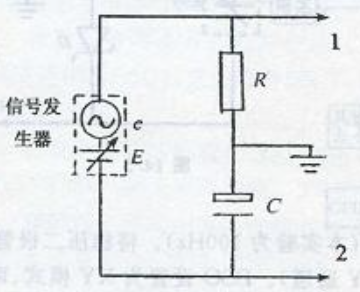
\includegraphics[width=5cm]{3.png} % 替换为你的图片路径
        \caption{动态电容值实验电路图}
    \end{minipage}\hfill
    \begin{minipage}{0.45\textwidth}
        \centering
        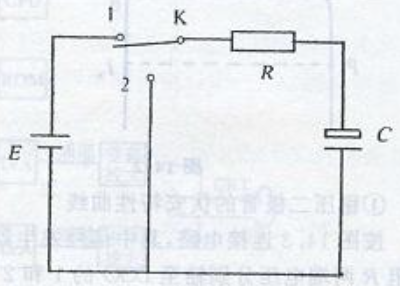
\includegraphics[width=5cm]{4.png} % 替换为你的图片路径
        \caption{静态电容值实验电路图}
    \end{minipage}
\end{figure}

\subsection{电解电容器的静态测量值}
利用直流电源对电解电容进行充、放电测出的电容值即为该电容的静态测量值。

如Figure 4,当开关$K$合“1”时,电源$E$通过$R$对$C$进行充电。充电完毕,将开关$K$合至“2”端,电容$C$则通过$R$放电。充、放电过程中电容上的电压$u_C$随时$t$的变化规律为:

$$
u_c=E(1-e^{-\frac{t}{\tau}})\qquad (充电)
$$
$$
u_c=Ee^{-\frac{t}{\tau}}\qquad (放电)
$$

式中$\tau=RC$,称为该电路的时间常数。它决定了电容充、放电时间的快慢,$\tau$越大,充、放电持续的时间越长。

我们通过示波器测量放电过程中,电解电容器两端电压从$E$下降到$0.368E$的时间即可得到时间常数$\tau$,进而求出电解电容器的静态测量值。

\section{实验仪器}
数字示波器、信号发生器、稳压二极管$D$、电解电容$C$、定值电阻$R_1=500\ \Omega$、$R_2=10000\ \Omega$。

\section{实验内容及数据}
\subsection{稳压二极管动态电阻的测量}
1.按实验电路图连接电路,$R=R_1=500\ \Omega$,$f=100\ Hz$。

2.将示波器设定为$XY$模式,将交流电压幅度调至最低,调节信号源直流旋钮,观察稳压二极管的伏安特性曲线。

3.调节信号源直流旋钮,使得工作电压$I_P=-10\ mA$。调节交流电压幅度至合适值。

4.利用示波器测量稳压二极管$D$和电阻$R$两端正弦波电压的峰-峰值$\widetilde{U_D}$和$\widetilde{U_R}$。

\begin{figure}[!ht]
    \centering
    \begin{minipage}{0.45\textwidth} % 调整宽度为总宽度的45%
        \centering
        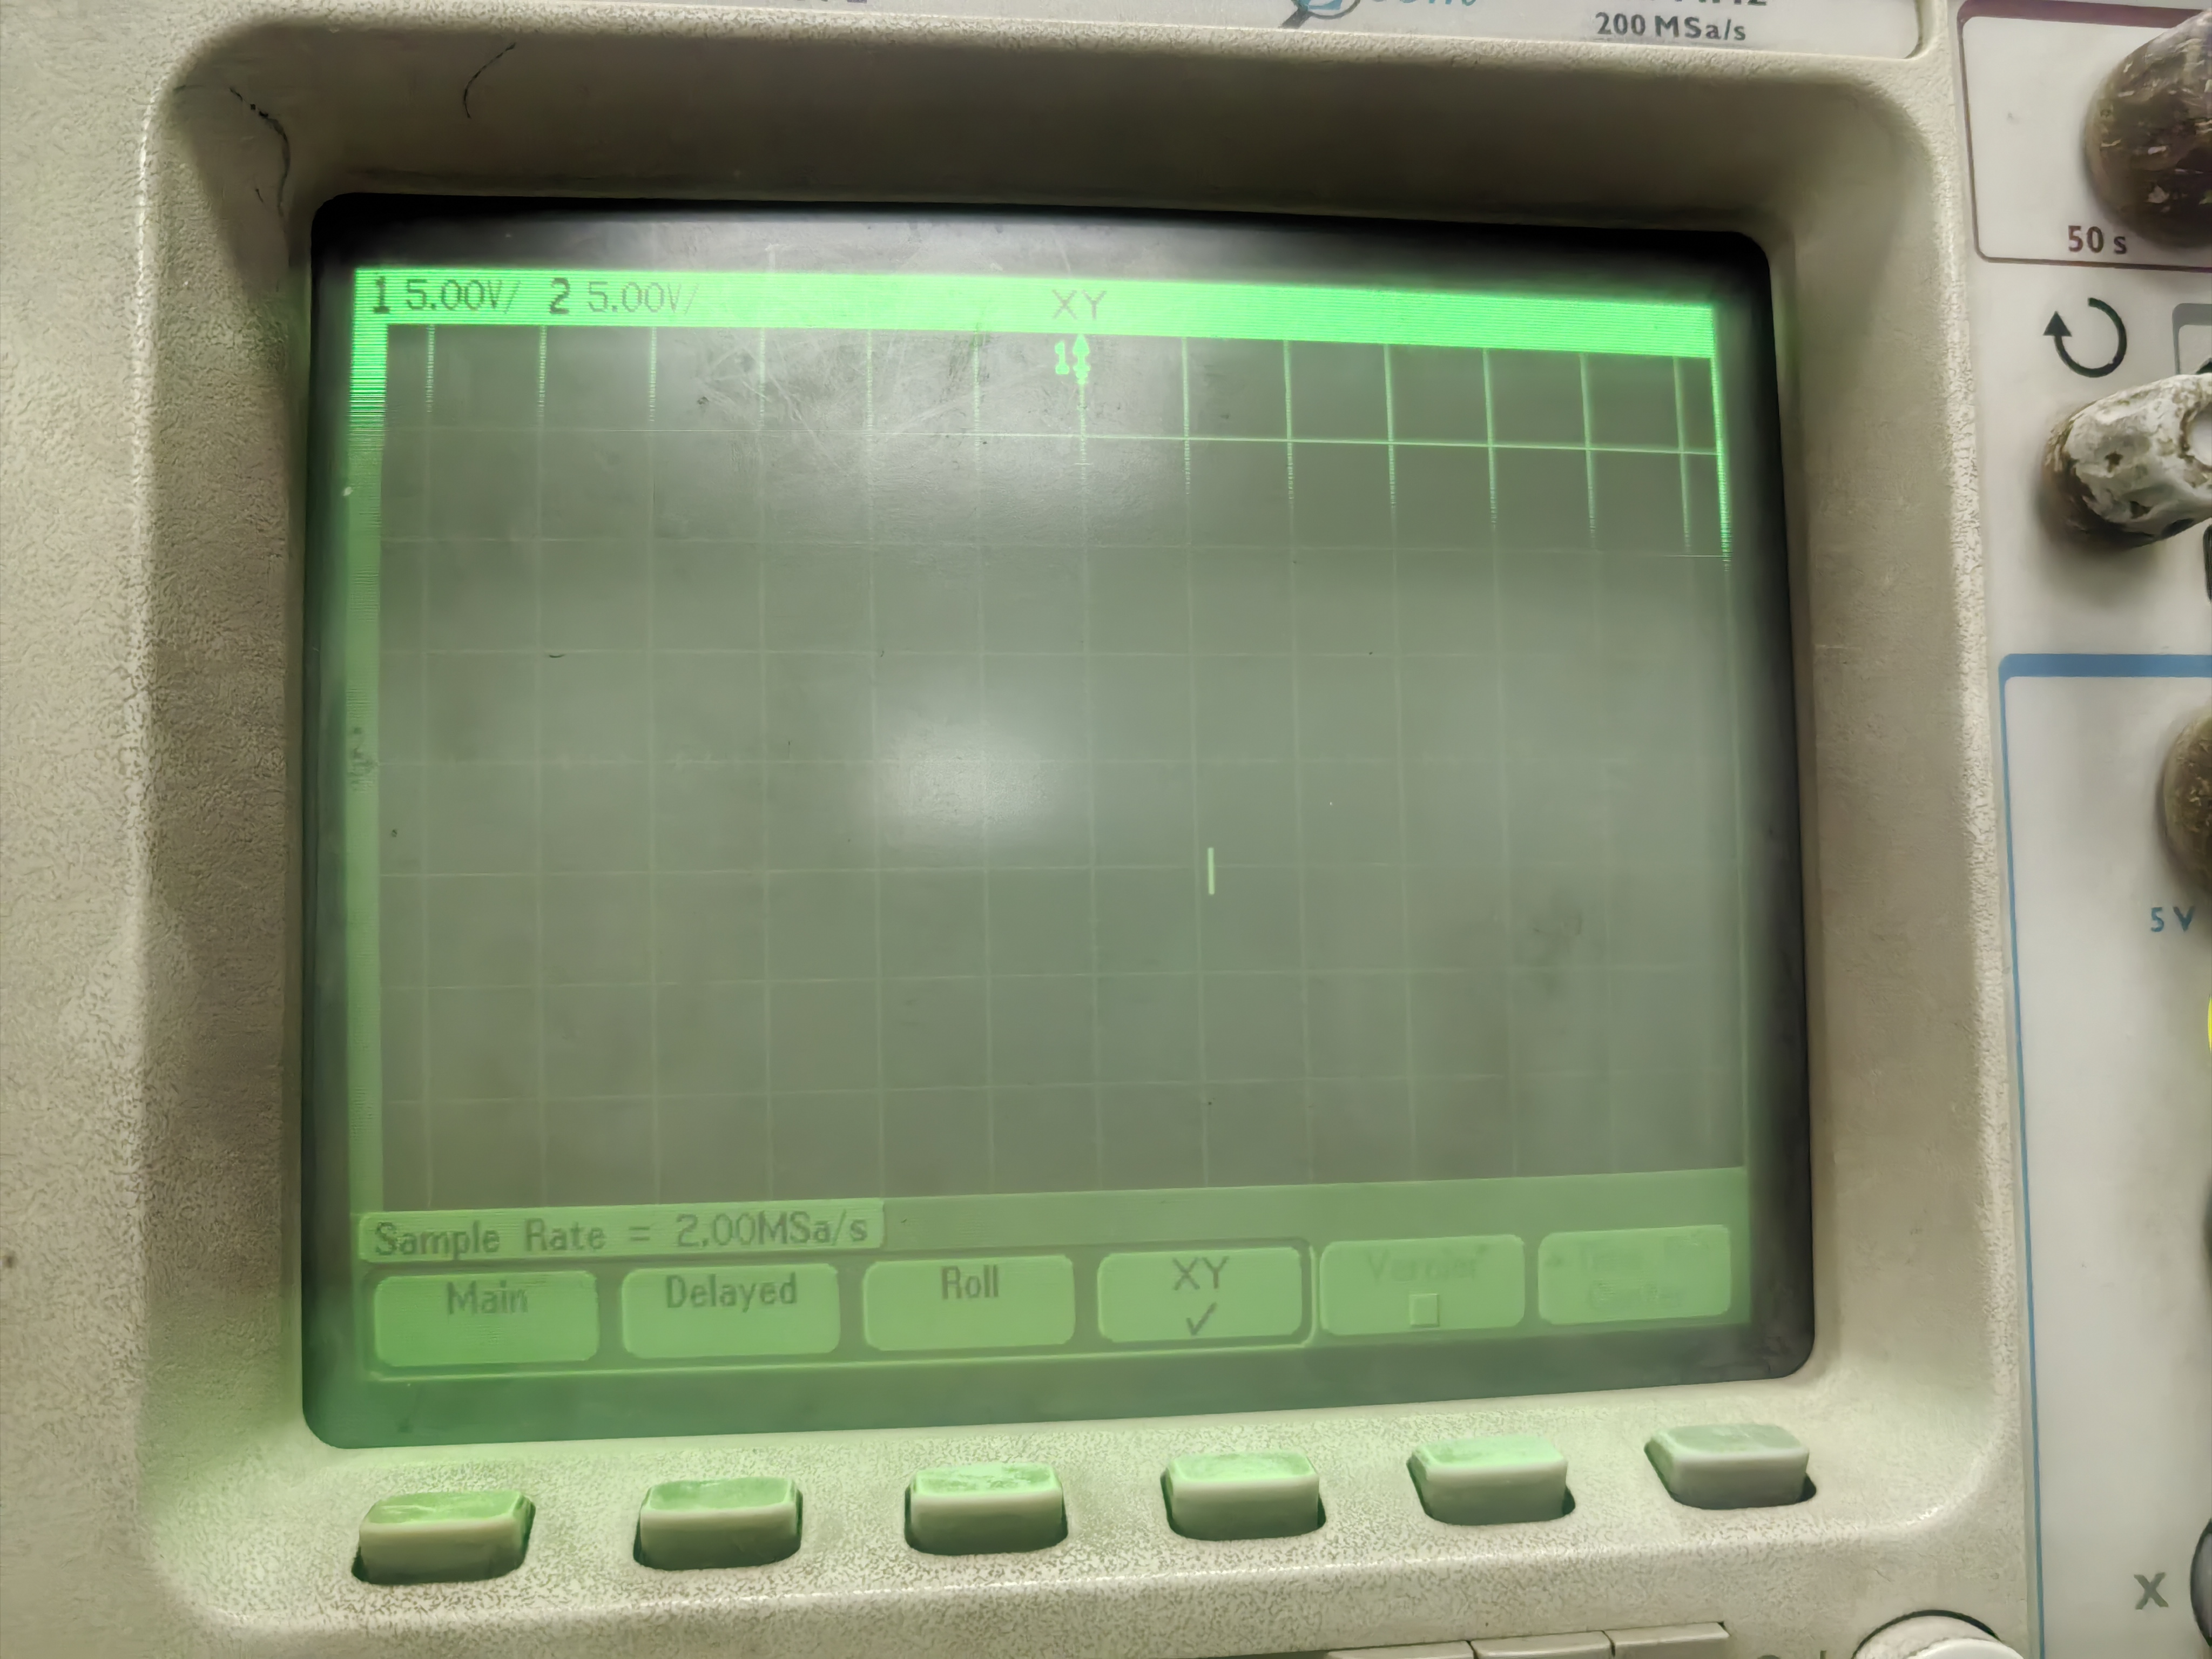
\includegraphics[width=7cm]{2.jpg} % 替换为你的图片路径
        \caption{稳压二极管的伏安特性曲线}
    \end{minipage}\hfill
    \begin{minipage}{0.45\textwidth}
        \centering
        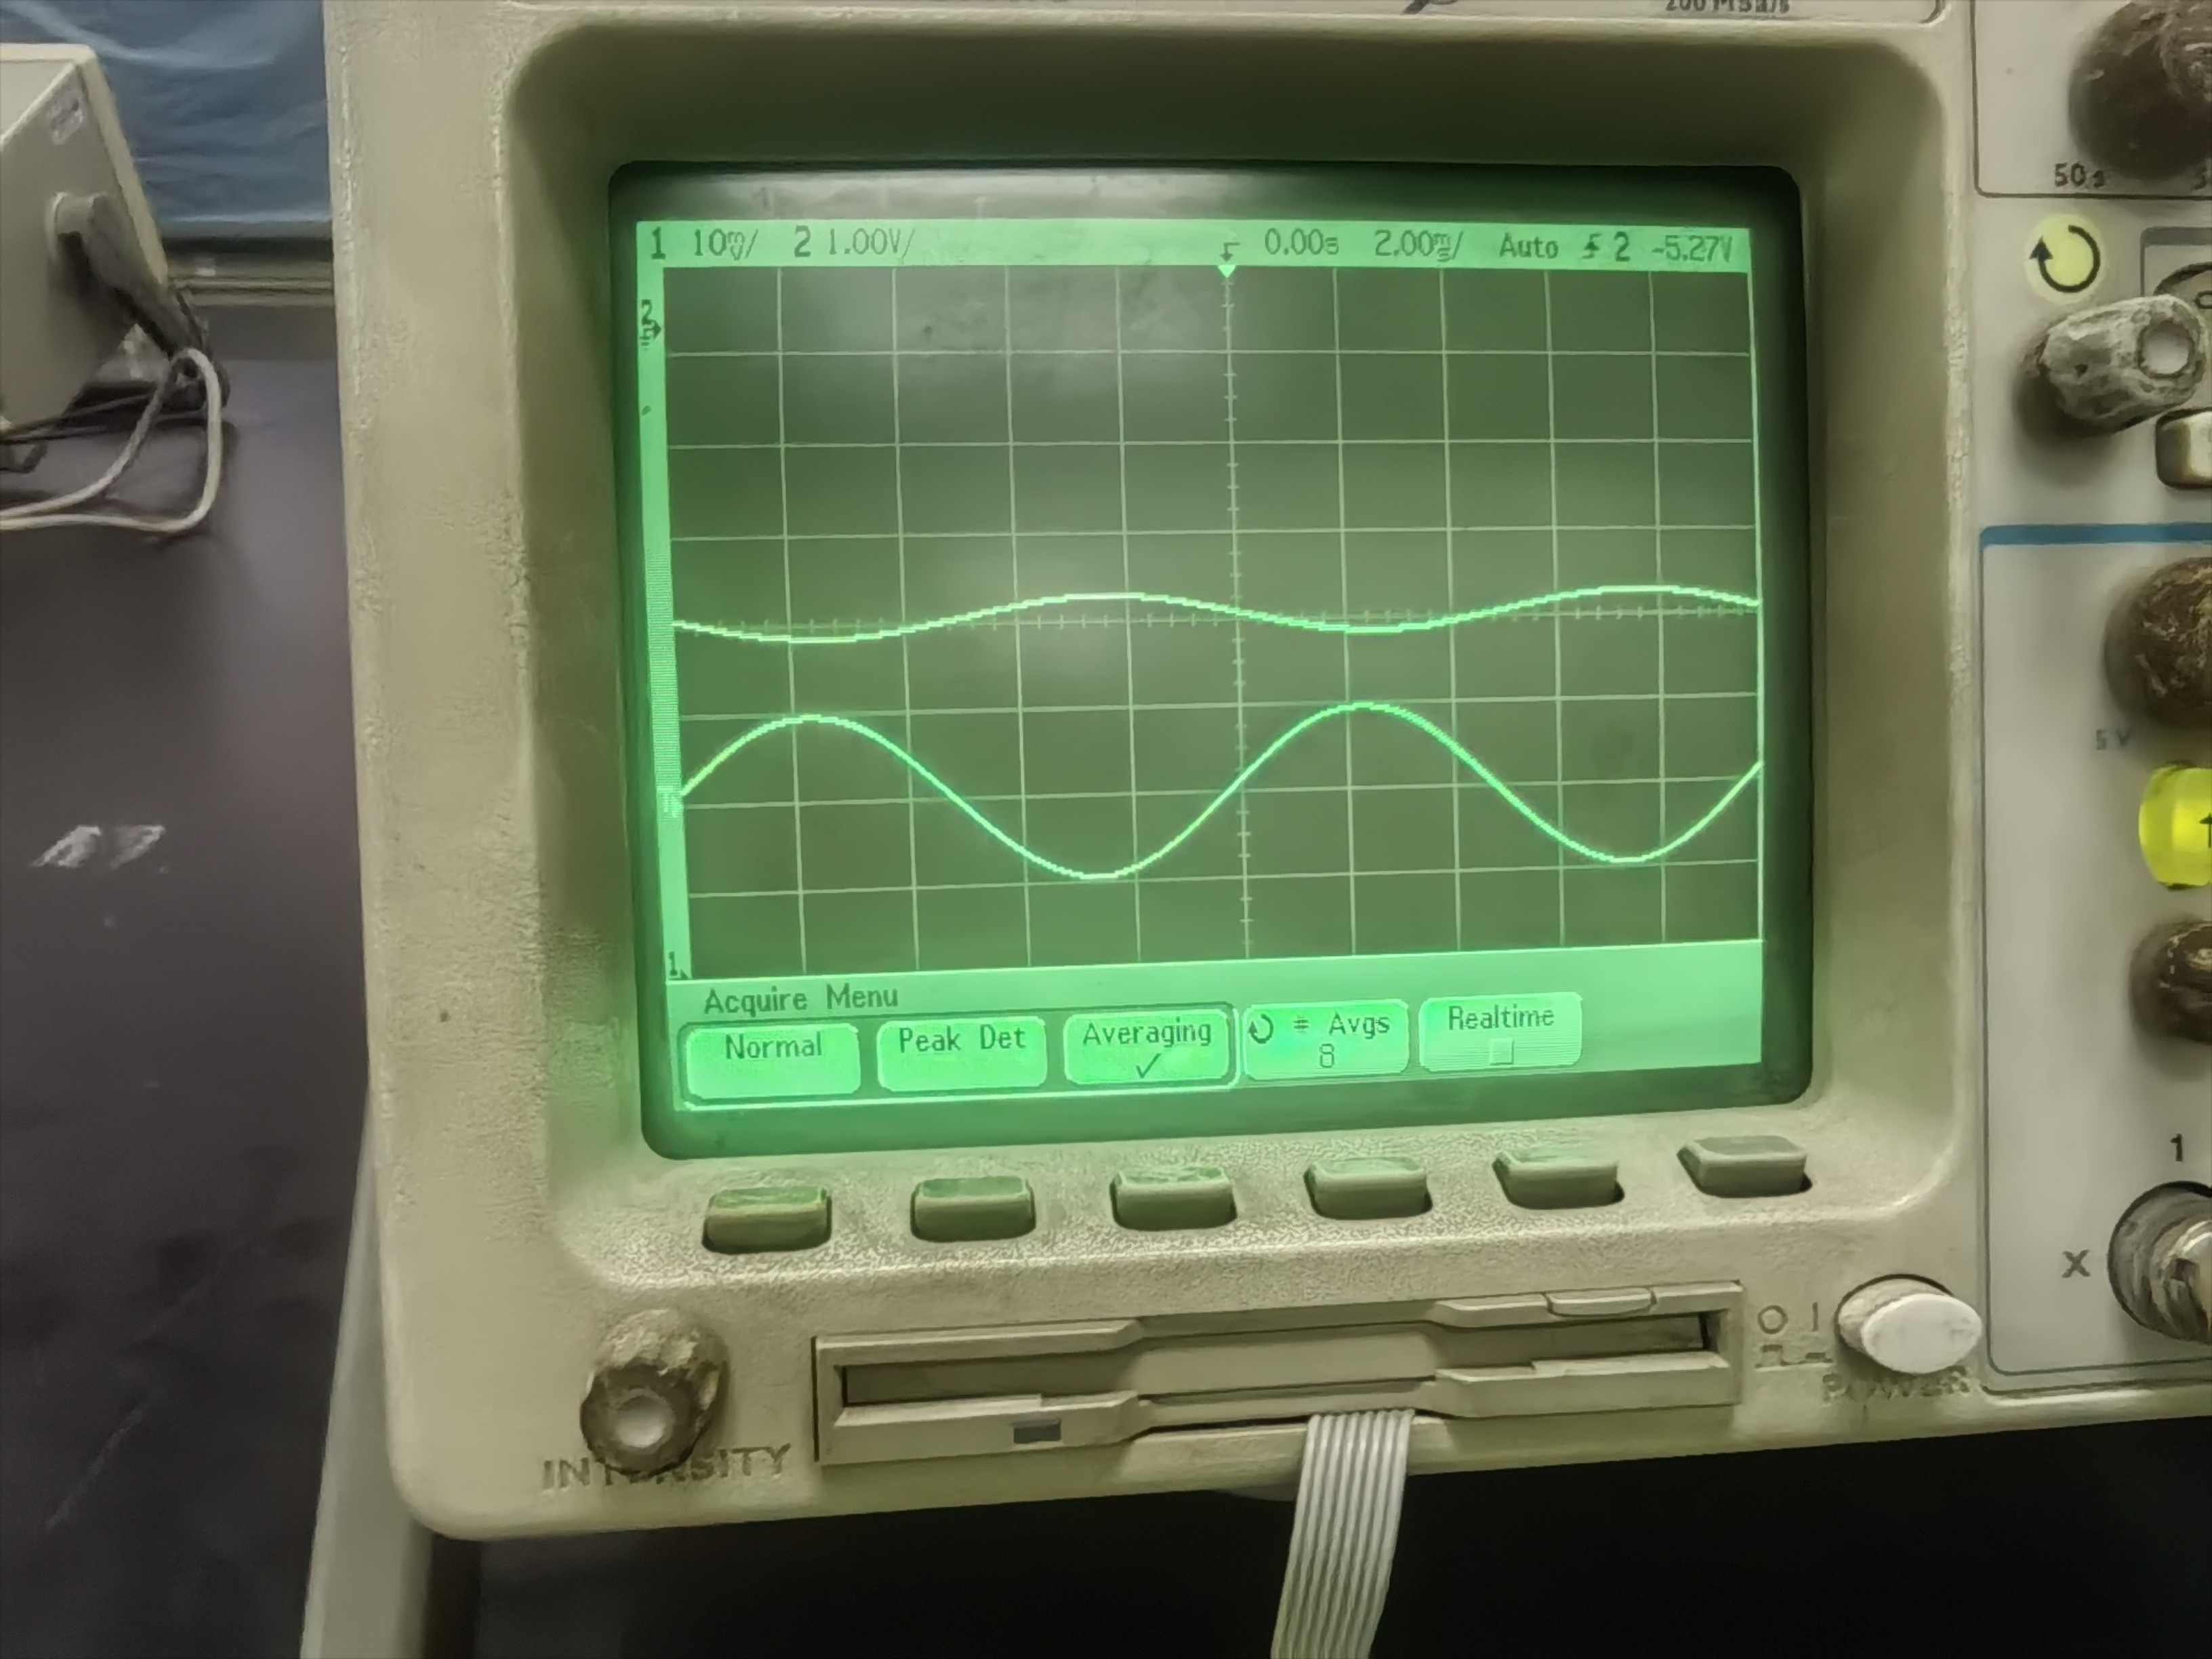
\includegraphics[width=7cm]{1.jpg} % 替换为你的图片路径
        \caption{稳态二极管$\widetilde{U_DD}$和$\widetilde{U_R}$}
    \end{minipage}
\end{figure}

得到:$\widetilde{U_D}=6.17\ mA$、$\widetilde{U_R}=2.6\ V$。计算得到稳压二极管动态电阻:

$$
\widetilde{r_{\backsim}}=\frac{\widetilde{U_D}}{\widetilde{U_R}}R=1.19\ \Omega
$$

\subsection{电解电容器的动态测量值}
1.按实验电路图连接电路,$R=R_1=500\ \Omega$,$f=100\ Hz$。

2.调节信号源直流调节旋钮,使得电解电容器两端的工作电压为$U_P=-10\ V$。

3.适当调节交流电压,测量电解电容$C$和电阻$R$两端交流电压的峰-峰值$\widetilde{U_C}$和$\widetilde{U_R}$。

\begin{figure}[!ht]
    \centering
    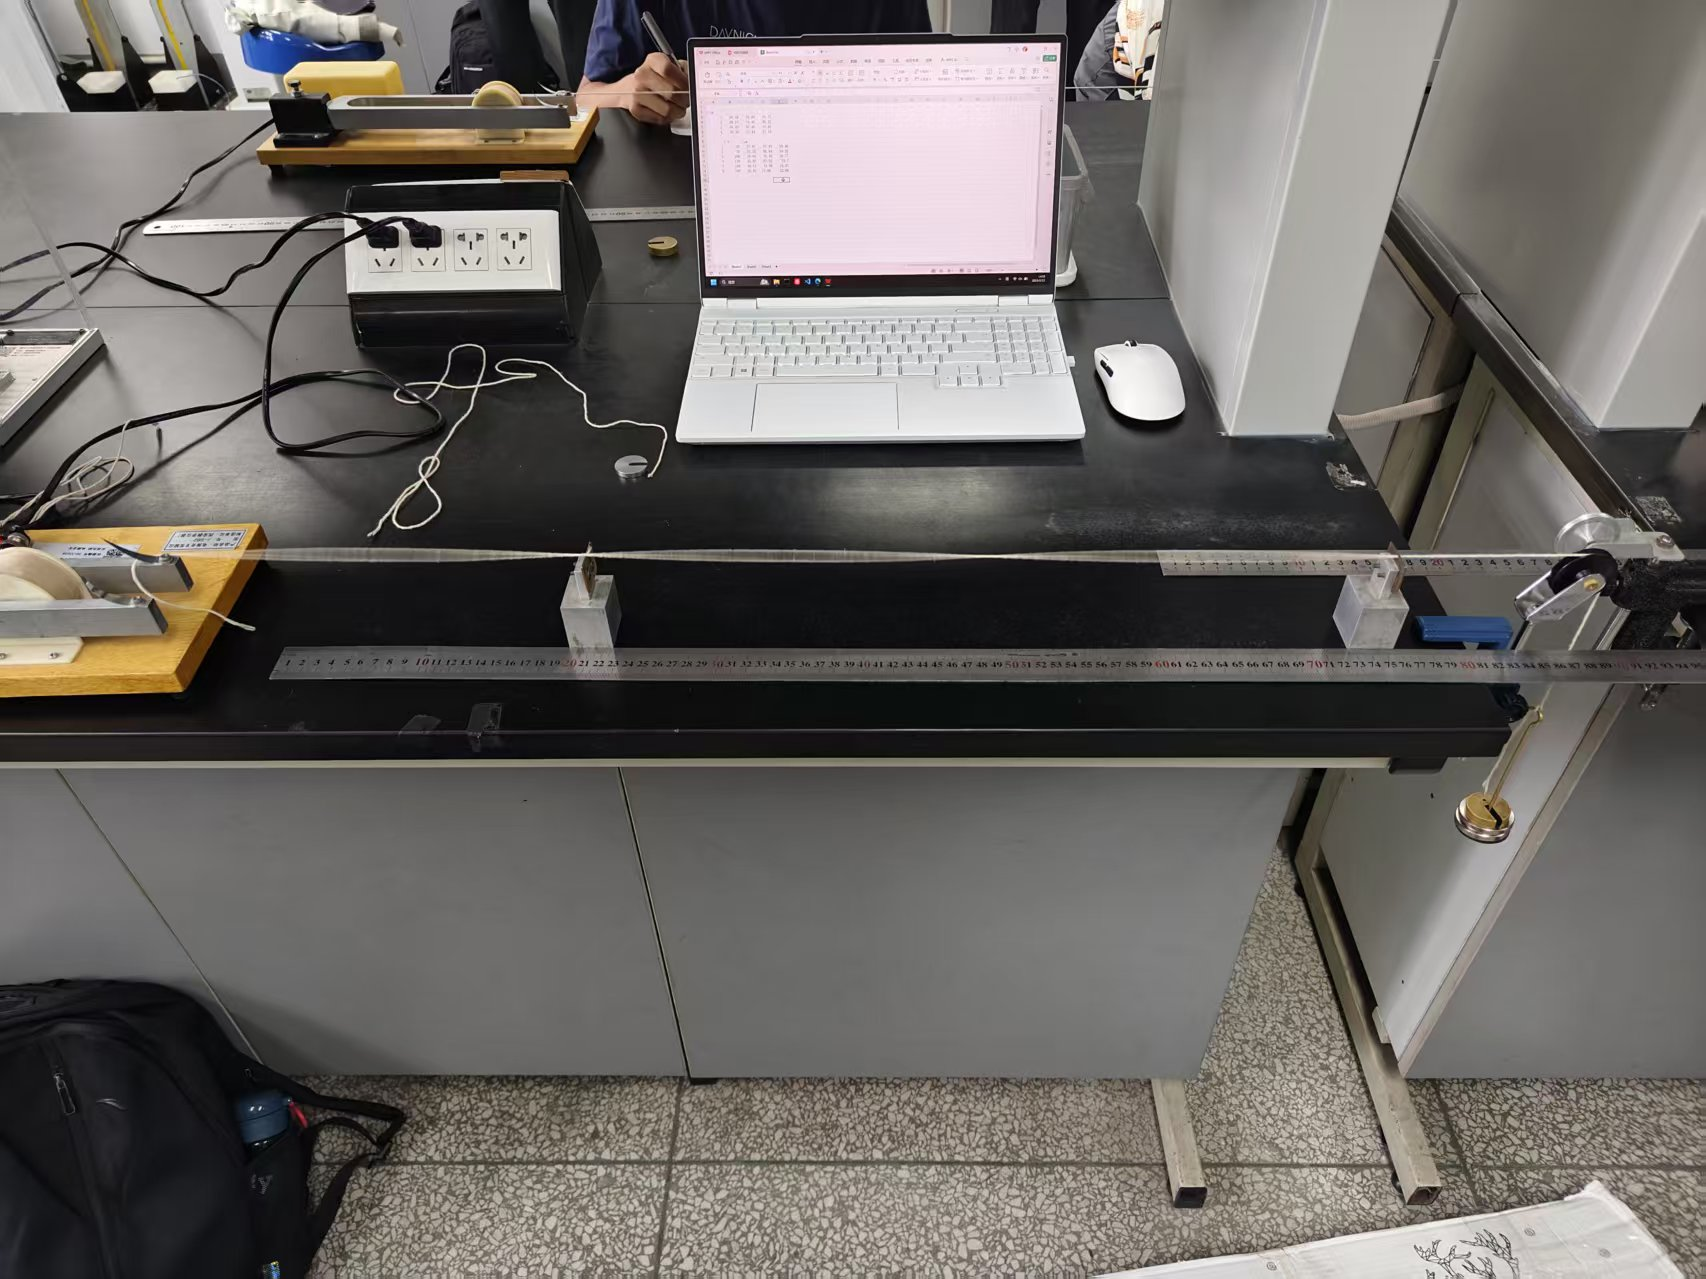
\includegraphics[width=7cm]{3.jpg}
    \caption{电解电容器$\widetilde{U_C}$和$\widetilde{U_R}$}
\end{figure}

得到:$\widetilde{U_C}=5.60\ mV$、$\widetilde{U_R}=1.641\ V$。计算得到电解电容器的动态测量值:

$$
C=\frac{\widetilde{U_R}}{2\pi f\widetilde{U_C}R}=933\ \mu F
$$

\subsection{电解电容器的静态测量值}
1.按实验电路图连接电路。$R=R_2=10000\ \Omega$。

2.设置数字示波器的扫描速度为10.0s,测量电解电容器的放电曲线。

3.通过示波器测量放电过程中,电解电容器两端电压从$E$下降到$0.368E$的时间得到时间常数$\tau$。

\begin{figure}[!ht]
    \centering
    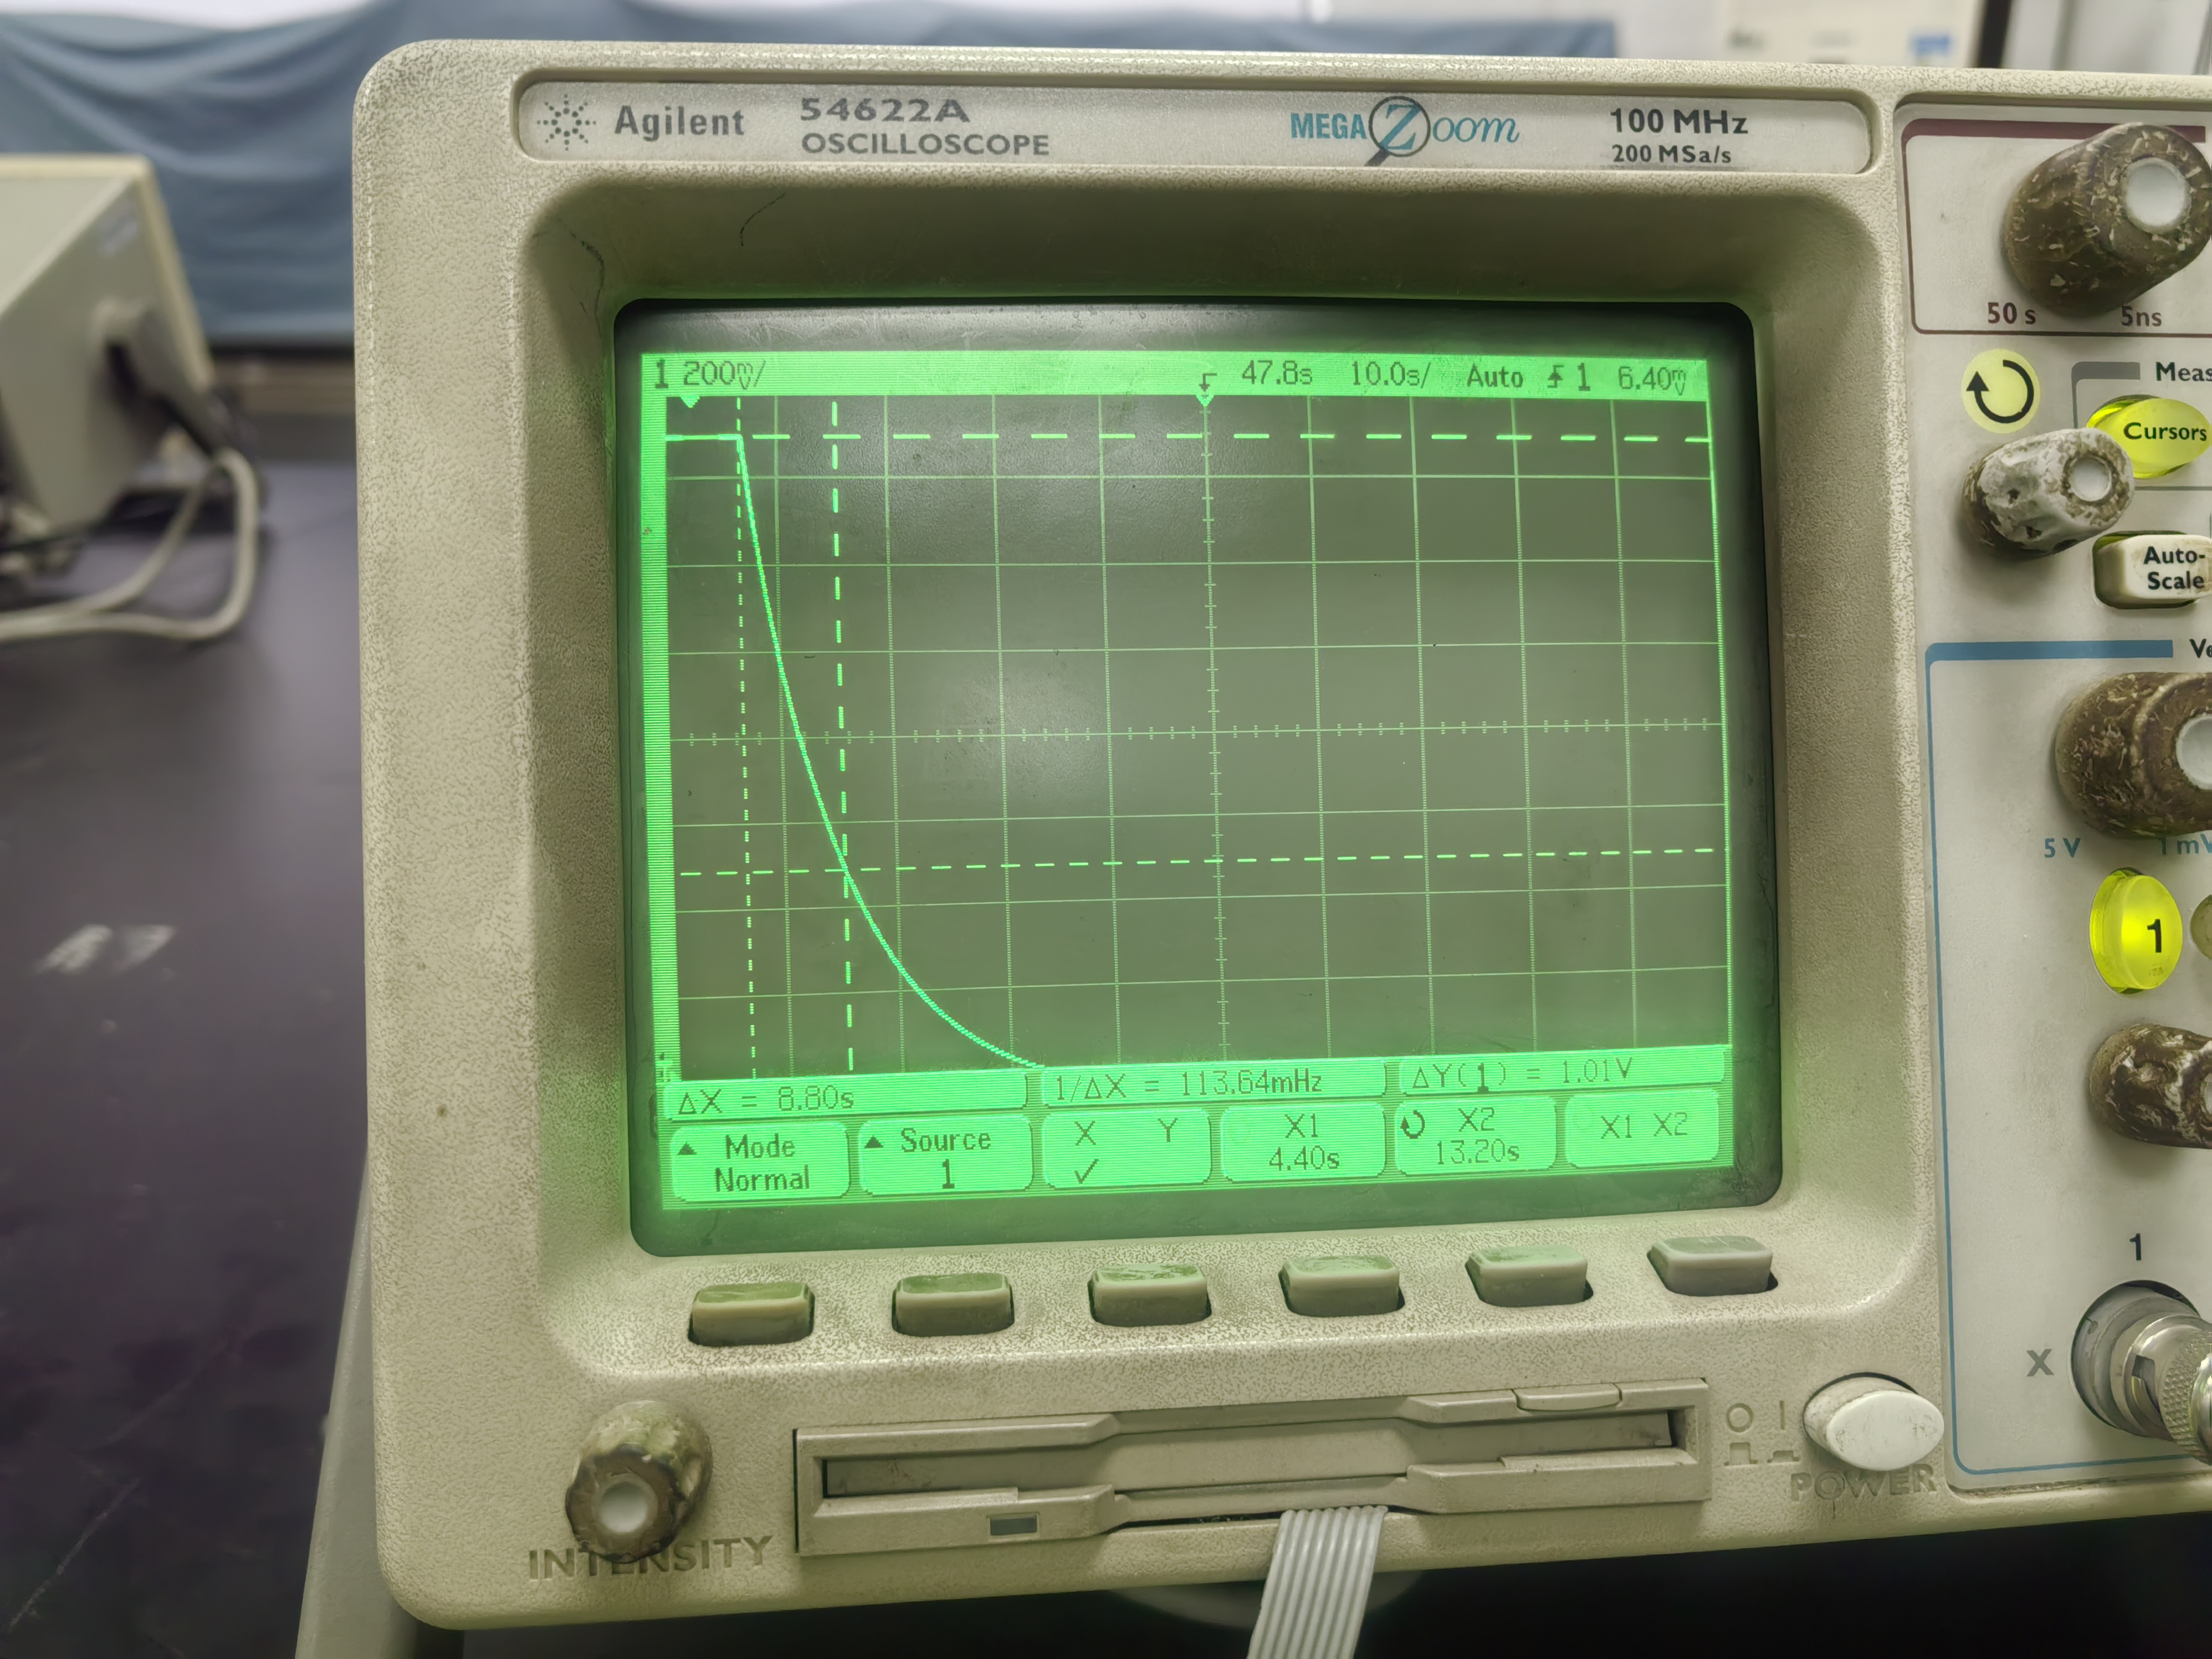
\includegraphics[width=7cm]{4.jpg}
    \caption{电解电容器放电曲线}
\end{figure}

得到:时间常数$\tau=8.80s$。计算得到电解电容器的静态测量值为:

$$
C=\frac{\tau}{R}=880\ \mu F
$$

\section{总结}
本次实验中,我们学习了数字示波器的使用方法,并得到了稳压二极管的伏安特征曲线和动态电阻,以及电解电容器的动态和静态测量值,对数字示波器的使用有了更加全面深刻的了解。
\end{document}